\documentclass[11pt,reqno]{amsart}
\usepackage[top=1in, left=1in, right=1in, bottom=1in]{geometry}                % See geometry.pdf to learn the layout options. There are lots.
\geometry{letterpaper}                   % ... or a4paper or a5paper or ... 
\usepackage[parfill]{parskip}    % Activate to begin paragraphs with an empty line rather than an indent
%\usepackage{algorithm, algorithmic}

\usepackage{algorithm}
\usepackage{algpseudocode}

\usepackage{graphicx}

\usepackage{verbatim}
\usepackage{amssymb}
\usepackage{amsmath}

\usepackage{enumitem}

\usepackage{setspace}
\doublespacing

\usepackage{natbib}

%\usepackage{epstopdf}
%\DeclareGraphicsRule{.tif}{png}{.png}{`convert #1 `dirname #1`/`basename #1 .tif`.png}

\newcommand{\RR}{I\!\!R} %real numbers
\DeclareMathOperator{\diag}{diag}

\algnewcommand{\Inputs}[1]{%
  \State \textbf{Inputs:}
  \Statex \hspace*{\algorithmicindent}\parbox[t]{.8\linewidth}{\raggedright #1}
}
\algnewcommand{\Initialize}[1]{%
  \State \textbf{Initialize:}
  \Statex \hspace*{\algorithmicindent}\parbox[t]{.8\linewidth}{\raggedright #1}
}

\title[RVD2]{RVD2: An ultra-sensitive variant detection model for low-depth targeted next-generation sequencing data}
\author{}
%\date{}                                           % Activate to display a given date or no date

\begin{document}

\begin{abstract}
Next-generation sequencing technology is increasingly being used for clinical diagnostic tests. Unlike most research samples, these clinical samples are often genomically heterogeneous due to low sample purity or the presence of genetic subpopulations. However, many variant calling algorithms are optimized to call single nucleotide polymorphisms in homogeneous rather than heterogeneous samples. We present a novel variant calling algorithm that uses a hierarchical Bayesian model to estimate allele frequency and a Bayesian posterior hypothesis test to call variants in heterogeneous samples. We show that our algorithm improves upon current classifiers and has higher sensitivity and specificity over a wide range of median read depths and a minor allele frequencies. We use our algorithm to call variants in a pooled sample of 100 patients with multiple sclerosis and identify novel variants in IL7RA and IL2R.
\end{abstract}

\maketitle

\section{Introduction}

Next-generation sequencing (NGS) technology has enabled the systematic interrogation of the genome for a fraction of the cost of traditional assays~\citep{Koboldt:2013kw}. Protocol and platform engineering improvements have enabled the generation of $1\times10^9$ bases of sequence data in 27 hours for approximately \$1000~\citep{Quail:2012hf}. As a result, NGS is increasingly being used as a general platform for research assays for methylation state~\citep{Laird:2010ab}, DNA mutations~\citep{Consortium:2013co}, copy number variation~\citep{Alkan:2009cr}, promoter occupancy~\citep{Ouyang:2009hc} and others~\citep{Rivera:2013ee}. NGS diagnostics are being translated to clinical applications including noninvasive fetal diagnostics~\citep{Kitzman:2012hea}, infectious disease diagnostics~\citep{Capobianchi:2012em}, cancer diagnostics~\citep{Navin:2010gu}, and human microbial analysis~\citep{Consortium:2013iz}. 

Clinical samples are often genetically heterogeneous. For example, non-invasive fetal DNA testing uses maternal blood sample to sequence the minority fraction of cell-free fetal DNA~\citep{Fan:2008di}. Infectious diseases such as HIV and influenza may contain many genetically heterogeneous sub-populations~\citep{Flaherty:2011ja, Ghedin:2010ie}. DNA sequencing of individual regions of a solid tumor has revealed genetic heterogeneous within an individual sample~\citep{Navin:2010gu}.  

However, the primary statistical tools for calling variants from NGS data are optimized for homogeneous samples. Most analysis pipelines make use of preprocessing or postprocessing or both to eliminate error prone reads and false positives. Samtools/bcftools and GATK a naive Bayes decision rule to call a variant~\citep{}. GATK involves more sophisticate pre and post-processing steps. The genotype prior is fixed and constant across all loci and the likelihood of an allele at a locus is a function of the phred score~\citep{McKenna:2010bv}.

Recently, researchers have developed algorithms to call low-frequency or rare variants in heterogeneous samples.  VarScan2 combines algorithmic heuristics to call genotypes in the tumor and normal sample pileup data and then applies a Fisher's exact test on the read count data to detect a significant difference in the genotype calls~\citep{Koboldt:2012cg}. Strelka uses a hierarchical Bayesian approach to model the joint distribution of the allele frequency in the tumor and normal samples at each locus~\citep{Saunders:2012fh}. With the joint distribution available, one is able to identify locations with dissimilar allele frequencies. muTect uses a Bayesian posterior probability in its decision rule to evaluate the likelihood of a mutation~\citep{Cibulskis:2013ta}.

The remainder of this paper presents a novel algorithm for calling rare variants in heterogeneous samples using NGS data that is an improvement upon currently available technology. We present the hierarchical Bayesian model in Section~\ref{sec:model_structure} and a Bayesian hypothesis test to detect mutations in Section~\ref{sec:hypothesis_test}. In Section~\ref{sec:read_depth} we present sensitivity and specificity results of our method on known, pure DNA samples mixed at defined fractions. We compare our algorithm to the most accurate methods available to date in Section~\ref{sec:comparison}. Finally, in Section~\ref{sec:ms} we present results on detecting mutations associated with multiple sclerosis from data obtained from pooling 100 affected patients~\citep{Ferretti:2013hp}.

\section{Materials and Methods}

RVD uses a two-stage approach for detecting for rare variants. First, it estimates the parameters of two hierarchical Bayesian models; one using data from the sample of interest (case) and one using data from a known reference sample (control). Then, it tests for a significant difference between model parameters in the case and control samples and returns called variant positions.

\subsection{Model Structure}\label{sec:model_structure}

For a given sample, the observed data consists of two matrices $r \in \RR^{J \times N}$ and $n \in \RR^{J \times N}$, where $r_{ji}$ is the number of reads with a non-reference base at location $j$ in experimental replicate $i$ and $n_{ji}$ is the total number of reads at location $j$ in replicate $i$. The generative process is as follows:

\begin{enumerate}[noitemsep]
	\item For each location $j$: 
	\begin{enumerate}
		\item Draw an error rate $\mu_j \thicksim \text{Beta}(\mu_0, M_0)$
		\item For each replicate $i$:
		\begin{enumerate}
			\item Draw $\theta_{ji} \thicksim \text{Beta}(\mu_j, M_j)$
			\item Draw $r_{ji} | n_{ji} \thicksim \text{Binomial}(\theta_{ji}, n_{ji})$
		\end{enumerate}
	\end{enumerate}
\end{enumerate}

This process involves several hyperparameters: $\mu_0$, a global error rate; $M_0$, a global precision; $M_j$, a local precision. The global error rate, $\mu_0$, estimates the expected error rate across all locations. The global precision, $M_0$, estimates the variation in the error rate  across locations. The local precision, $M_j$, estimates the variation in the error rate across replicates at location $j$.

RVD2 has three levels of sampling. First, a global error rate and global precision are chosen once for the entire data set. Then, at each location, a local precision is chosen and a local error rate is sampled from a beta distribution. Finally, the error rate for replicate $i$ at location $j$ is drawn from a beta distribution and the number of non-reference reads is drawn from a binomial.

RVD2 hierarchically partitions sources of variation in the data. $r_{ji} | n_{ji} \thicksim \text{Binomial}(\theta_{ji}, n_{ji})$ models the variation due to sampling the pool of DNA molecules on the sequencer. $\theta_{ji} \thicksim \text{Beta}(\mu_j, M_j)$ models the variation due to experimental reproducibility. The variation in error rate due to sequence context is modeled by $\mu_j \thicksim \text{Beta}(\mu_0, M_0)$. Importantly, increasing the read depth $n_{ji}$ only reduces the sampling error, but does nothing to reduce experimental variation or variation due to sequence context.

\begin{figure}[h]
\begin{center}
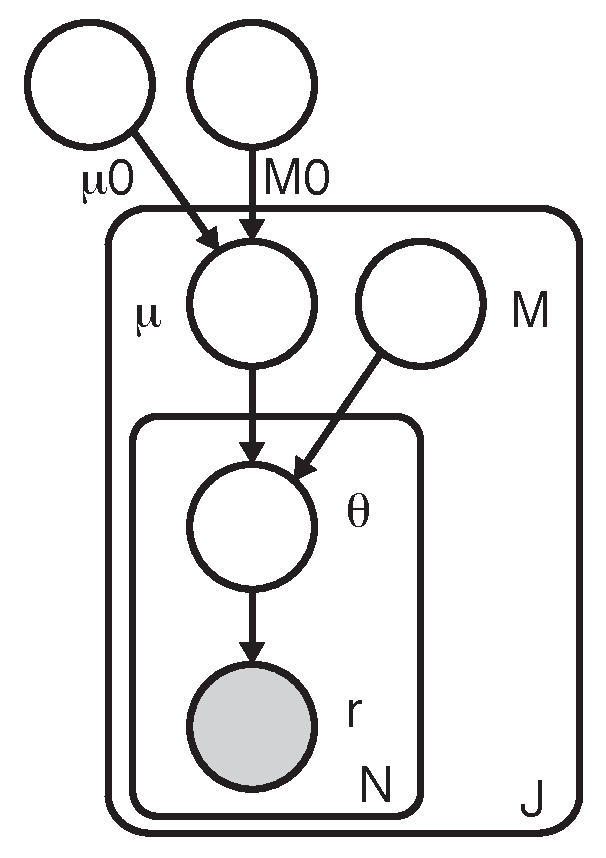
\includegraphics[width=40mm]{pdf_figs/RVD2_model.pdf}
\caption{RVD2 Graphical Model}
\label{fig:graphical_model}
\end{center}
\end{figure}

Figure~\ref{fig:graphical_model} shows a graphical representation of the RVD2 statistical model. In this graphical model framework a shaded node represents an observed random variable, an unshaded node represents an unobserved or latent random variable and a directed edge represents a functional dependency between the two connected nodes~\cite{}. A rounded box or ``plate" represents replication of the nodes within the plate. This graphical model framework connects graph theory and probability theory in a way that facilitates algorithmic methods for statistical inference.

The joint distribution over the latent and observed variables for data at location $j$ in replicate $i$ given the parameters is

\begin{equation}\label{eqn:jointpdf}
p \left( r_{ji}, \theta_{ji}, \mu_j | n_{ji}; \mu_0, M_0, M_j \right) = p \left( r_{ji} | \theta_{ji}, n_{ji} \right) p\left( \theta_{ji} | \mu_j; M_j \right) p\left( \mu_j; \mu_0, M_0 \right)
\end{equation}

\begin{gather}
= \frac{ \Gamma(M_0) } { \Gamma(\mu_0 M_0) \Gamma(M_0 (1-\mu_0)) } \mu_j^{M_0\mu_0 -1} (1 - \mu_j)^{M_0 ( 1 - \mu_0) - 1} \\
\cdot \frac{ \Gamma(M_j) } { \Gamma(\mu_j M_j) \Gamma(M_j (1-\mu_j)) } \theta_{ji}^{M_j\mu_j -1} (1 - \theta_{ji})^{M_j ( 1 - \mu_j) - 1} \\
\cdot \frac{ \Gamma(n_{ji}+1) } { \Gamma(r_{ji}+1) \Gamma( n_{ji} - r_{ji} + 1 ) } \theta_{ji}^{r_{ji}} (1 - \theta_{ji})^{n_{ji} - r_{ji}}
\end{gather}

Integrating over the latent variables $\theta_{ji}$ and $\mu_j$ yields the marginal distribution of the data at location $j$ in replicate $i$, 
\begin{equation}
p \left( r_{ji} | n_{ji} ; \mu_0, M_0, M_j \right) = \int_{\mu_j} \int_{\theta_{ji}}  p \left( r_{ji} | \theta_{ji}, n_{ji} \right) p\left( \theta_{ji} | \mu_j; M_j \right) p\left( \mu_j; \mu_0, M_0 \right) d\theta_{ji} d\mu_j
\end{equation}

Finally, the complete likelihood is

\begin{equation}
p \left( r ; \mu_0, M_0, M \right) = \prod_{j=1}^J p\left( \mu_j; \mu_0, M_0 \right) \prod_{i=1}^N p \left( r_{ji} | \theta_{ji}, n_{ji} \right) p\left( \theta_{ji} | \mu_j; M_j \right) 
\end{equation}

\section{Inference and Hypothesis Testing}

The primary object of inference in this model is the joint posterior distribution function over the latent variables,
\begin{equation}
	p(\mu, \theta | r, n; \phi)  = \frac{ p(\mu, \theta, r | n; \phi) } {p ( r | n; \phi)},
\end{equation}
where the parameters are $\phi \triangleq \{\mu_0, M_0, M\}$.

Exact inference in this model is intractable due to the coupling between the local and global beta distributions. [XXX complete this proof] 

Instead, we have developed a Metropolis-within-Gibbs  approximate inference algorithm shown in Algorithm~\ref{alg:metro_gibbs}. First, the hyperparameters are initialized using method-of-moments. Given those hyperparameter estimates, we sample from the marginal posterior distribution for $\mu_j$ given its Markov blanket using a Metropolis-Hasting rejection sampling rule. Finally, we sample from the marginal posterior distribution for $\theta_{ji}$ given its Markov blanket. Samples from $\theta_{ji}$ can be drawn from the posterior distribution directly  because the prior and likelihood form a conjugate pair. This sampling procedure is repeated until the chain converges to a stationary distribution then we draw samples from the posterior distribution over latent variables.

\begin{algorithm}[ht]
\caption{Metropolis-within-Gibbs Algorithm}
\label{alg:metro_gibbs}
\begin{algorithmic}[1]

\State Initialize $\theta$, $\mu$, $M$, $\mu_0$, $M_0$
\Repeat
\For {each location j} \Comment{Sample $\mu_j$}
  \State Draw T samples from $p \left( \mu_j |\theta_{ij},\mu_0,M_0\right)$ using M--H
  \State Set $\mu_j$ to the sample median for the T samples
  
  
  \For {each replicate i} \Comment{Sample $\theta_{ji}$}
	\State Sample from $p \left( \theta_{ij} |r_{ij},n_{ij},\mu_j,M \right)$
  \EndFor

\EndFor
\Until {sample size sufficient}
\end{algorithmic}
\end{algorithm}

%%%%%%%%%%%%%
% Initialization
%%%%%%%%%%%%%
\subsection{Initialization}
The initial values for the model parameters and latent variables is obtained by a method-of-moments (MoM) procedure. MoM works by setting the population moment equal to the sample moment. A system of equations is formed such that the number of moment equations is equal to the number of unknown parameters and the equations are solved simultaneously to give the parameter estimates. We simply start with the data matrices $r$ and $n$ and work up the hierarchy of the graphical model solving for the parameters of each conditional distribution in turn.

We present the initial parameter estimates here and provide the derivations in Appendix~\ref{sec:appendix_mom}. The MoM estimate for replicate-level parameters are $\tilde{\theta}_{ji} = \frac{r_{ji}} {n_{ji}}$. The estimates for the position-level parameters are $\tilde{\mu}_j = \frac{1}{N} \sum_{i=1}^N \theta_{ji}$ and $\tilde{M_j} = \frac{ \tilde{\mu}_j (1 - \tilde{\mu}_j ) } { \frac{1}{N} \sum_{i=1}^N \theta_{ji}^2 } -1$. The estimates for the genome-level parameters are $\tilde{\mu}_0 = \frac{1}{J} \sum_{j=1}^J \mu_j$ and $\tilde{M}_0 = \frac{ \tilde{\mu}_0 (1 - \tilde{\mu}_0 ) } {\frac{1}{J} \sum_{j=1}^J \mu_j^2 } -1$. While MoM is known to have the potential to return estimates outside the true parameter bounds, we have not encounter such pathological behavior in this application. 

%%%%%%%%%%%%%%%%%%
% Sampling theta
%%%%%%%%%%%%%%%%%%
\subsection{Sampling from $p \left( \theta_{ij} |r_{ij},n_{ij},\mu_j,M \right)$}

Samples from the posterior distribution $p(\theta_{ji} | r_{ji}, n_{ji}, \mu_j, M_j)$ are drawn analytically because of the Bayesian conjugacy between the prior $p(\theta_{ji} | \mu_j, M_j) \thicksim \text{Beta}(\mu_j, M_j)$ and the likelihood $p(r_{ji} | n_{ji}, \theta_{ji}) \thicksim \text{Binomial}(\theta_{ji}, n_{ji})$. The posterior distribution is 

\begin{equation}
	p(\theta_{ji} | r_{ji}, n_{ji}, \mu_j, M_j) \thicksim \text{Beta}\left( \frac{r_{ji} + M_j \mu_j}{n_{ji} + M_j} , n_{ji} + M_j\right).
\end{equation}

%%%%%%%%%%%%%%%%%%
% Sampling mu
%%%%%%%%%%%%%%%%%%
\subsection{Sampling from $p \left( \mu_j |\theta_{ji},\mu_0,M_0\right)$}
The posterior distribution over $\mu_j$ given its Markov blanket is 
\begin{equation}
	p( \mu_j | \theta_{ji}, M_j, \mu_0, M_0 ) \propto p(\mu_j | \mu_0, M_0) p(\theta_{ji} | \mu_j, M_j).
\end{equation}

Since the prior, $p(\mu_j | \mu_0, M_0)$, is not conjugate to the likelihood, $p(\theta_{ji} | \mu_j, M_j)$, we cannot write an analytical form for the posterior distribution. Instead, we sample from the posterior distribution using the Metropolis-Hastings algorithm.

A candidate sample is generated from the symmetric proposal distribution $Q(\mu_j^* | \mu_j^{(p)}) \thicksim $. The acceptance probability is then
\begin{equation}
	a = \frac{ p(\mu_j^* | \mu_0, M_0) p(\theta^{(p+1)}_{ji} | \mu_j^*, M_j) } {p(\mu_j^{(p)} | \mu_0, M_0) p(\theta^{(p+1)}_{ji} | \mu_j^{(p)}, M_j)}
\end{equation}

Since, each position $j$ is exchangeable given the global hyperparameters $\mu_0$ and $M_0$ this algorithm can be distributed across $J$ processors. We have found that the algorithm performance improves when we take the median of ten or more M-H samples as a single Gibbs step for each position. This computational effort only minimally increases run time when run on a parallel computing platform. In the experiments, we use a XX sample burn-in to allow the Markov chain to approach its stationary distribution and we thin the chain by a factor of 2 to reduce autocorrelation among samples.

%%%%%%%%%%%%%%%%%%
% Posterior Density Test
%%%%%%%%%%%%%%%%%%
\subsection{Hypothesis Test}\label{sec:hypothesis_test}
Metropolis-within-Gibbs provides samples from the posterior distribution of $\mu_j$ for both the control and case data. For notational simplicity, we define the random variables associated with these two distributions $\tilde{\mu}_j^{\text{case}}$ and $\tilde{\mu}_j^{\text{control}}$.

A variant is called if $\tilde{\mu}_j^{\text{case}} > \tilde{\mu}_j^{\text{control}}$ with high confidence,
\begin{equation}
	\Pr( \tilde{\mu}_j^{\text{case}} - \tilde{\mu}_j^{\text{control}} \geq \tau ) > 1-\alpha,
\end{equation}
where $\tau$ is a detection threshold and $1-\alpha$ is a confidence level. We draw a sample from the posterior distribution $\tilde{\mu}_j^{\Delta} \triangleq \tilde{\mu}_j^{\text{case}} - \tilde{\mu}_j^{\text{control}}$ by randomly sampling with replacement from the samples of $\tilde{\mu}_j^{\text{case}}$ and $\tilde{\mu}_j^{\text{control}}$.

The threshold, $\tau$, may be set to zero or optimized for a given median depth and desired MAF detection limit. The optimal $\tau$ maximizes the Matthews correlation coefficient.
\begin{equation}
	\tau^* = \arg\max_\tau \text{MCC}(\tilde{n}, \text{MAF})
\end{equation}


%%%%%%%%%%%%%%%%%%

% Chi^2 Test

%%%%%%%%%%%%%%%%%%
%\subsection{$\chi^2$ test for non-uniform base distribution}
%
%We assume the counts for the non-reference bases at poisiuton $j$ in replicate $i$ follow a multinomial distribution with parameter  $p = (p_1, p_2, p_3)$ where $p_k \geq 0$ for $k =1, 2, 3$ and $\sum_{k=1}^3 p_k = 1$.
%
%The non-reference reads may be due to a true mutation or due to a random sequencing error. We assume, non-reference read counts caused by a random mechanism results in a uniform distributed among three non-reference categories, giving $p_1=p_2=p_3=1/3$. In contrast, the distribution of non-reference read counts among three non-reference categories caused by mutation would be biased to one base. 
%
%We use a $\chi^2$ goodness-of-fit test to distinguish these two possible scenarios. The null hypothesis is $H_0: p = (p_1, p_2, p_3)$ where $p_1=p_2=p_3=1/3$. Cressie and Read (1984) identified a power-divergence family of statistics, indexed by $\lambda$, that includes as special cases Pearson's $\chi^2 (\lambda = 1)$ statistics, the log likelihood ratio statistics $(\lambda = 0)$, the Freeman-Tukey statistics $(\lambda = -1/2)$ the Neyman modified $X^2 (\lambda = -2)$. The test statistic is
%
%\begin{equation}
% 2nI^\lambda = \frac{2}{\lambda(\lambda+1)}\sum_{k=1}^3 r_{ji}^{(k)} \left[\left(\frac{r_{ji}^{(k)}}{E_{ji}^{(k)}}\right)^\lambda-1\right];\lambda \in R,
%\end{equation}
%
%where $r_{ji}^{(k)}$ is the observed frequency for non-reference base $k$ at position $j$ in replicate $i$ and $E_{ji}^{(k)}$ is the corresponding expected frequency under the null hypothesis. Cressie and Read (1984) proved that when $\lambda = 2/3$ this statistic is XXX.
%
%For each position, there are $N$ power-divergence statistics for each experimental replicate. We use Fisher's combined probability test to combine the p-values from each replicates into a single one for each position,
%
%\begin{equation}
%	X^2 = -2 \sum_{i=1}^N \ln(p_i).
%\end{equation}
%This gives a test statistic that follows a $\chi^2$ distribution with $2*N$ degrees of freedom when the null hypothesis is true.
%
%While Fisher's combined probability test collapses the p-values across replicates, we still have $J$ tests across positions. We use the Bejamini-Hochberg method to control the family-wise error rate (FWER) across positions.


\section{Results}

\subsection{Performance with read depth}\label{sec:read_depth}

We synthesized a 400bp control DNA sequence and another 400bp sequence that is identical to the control except at 14 loci with variant bases. We denote the indices of these true positive variant positions $j^*$. Pure case and control samples were mixed at defined fractions to yield minor allele frequencies (MAFs) of 0.1\%, 0.3\%, 1\%, 10\%, and 100\%. The sequencing protocol and data set are available from the original publication~\cite{}.

BAM files for the synthetic DNA data were down sampled by $10\times$, $100\times$, $1,000\times$, $10,000\times$ to simulate lower coverage data while retaining the error structure of real NGS data. The final data set contains pairs of reads for three replicates of each case and a pair of reads for the control sample giving a total of 36 BAM files for each downsampled data set.

We ran the RVD2 algorithm on each downsampled data set sand varied the threshold $\tau$ with fixed $\alpha=0.05$ to generate receiver operating characteristic (ROC) curves in Figure~\ref{fig:ROC}. Figure~\ref{ig:ROC}A shows ROC curves for a true 0.1\% MAF for a range of median coverage depths. At the lowest depth the sensitivity and specificity is no better than a random decision. We would not expect to be able to call a 1 in 1000 variant base with a coverage of only 43. The performance improves monotonically and is much better at a depth of approximately 41,000. This depth exceed the inverse MAF by a $10\times$ which we find to be generally a good coverage threshold for detecting variants. We find a similar pattern in Figures~\ref{fig:ROC}B-C. Interestingly, the algorithm performance is much better than a random decision rule to detect a 10\% MAF with only a depth of 25.

\begin{figure}[htbp]
\begin{center}
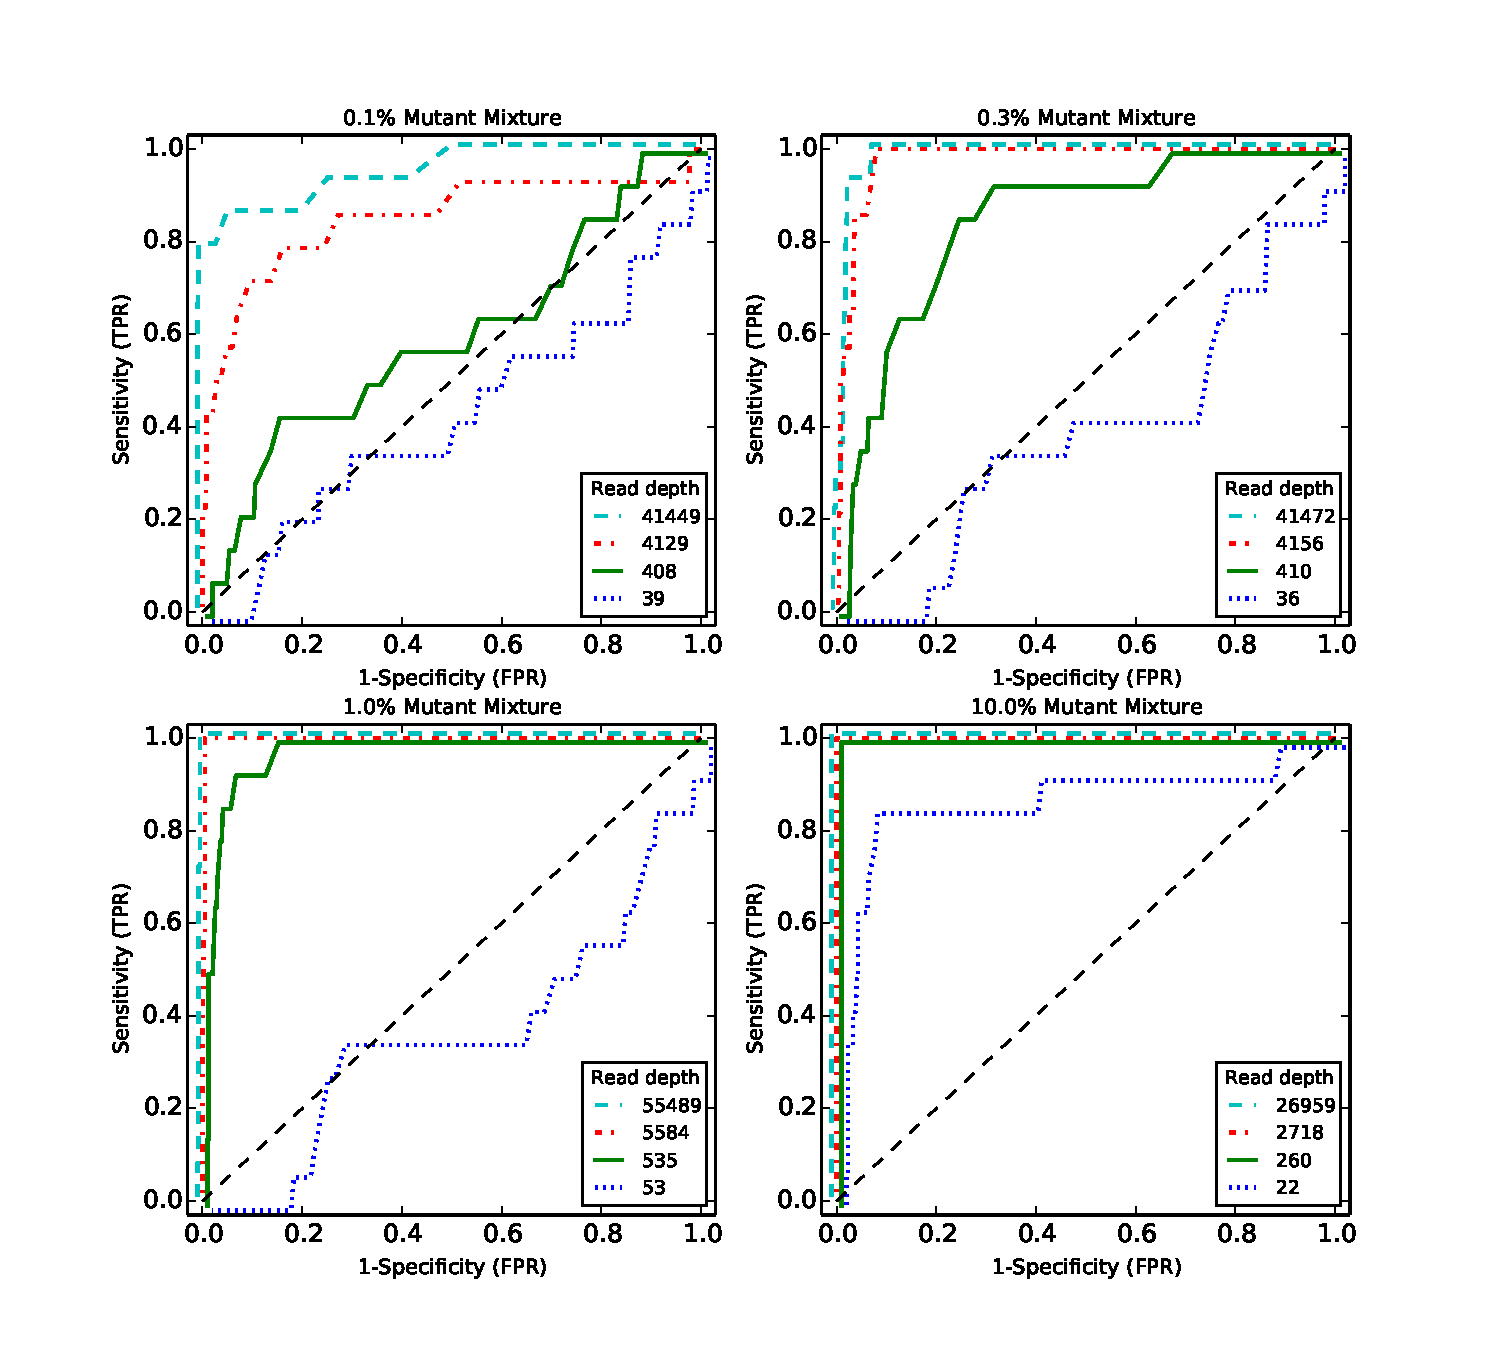
\includegraphics[width=120mm]{pdf_figs/ROC_without_chi2.pdf}
\caption{ROC curve varying read depth showing detection performance of model with Bayesian Hypothesis Test.}
\label{fig:ROC}
\end{center}
\end{figure}

Figure~\ref{fig:MAF} shows the posterior mean and 95\% credible intervals for $\mu_j$ for called variant positions with $\bar{n} = 41,573$. The only false positive is at position 8, though posterior distributions for the case and control clearly show a difference at that position. The posterior mean estimates are shrunken towards the global error rate parameter $\mu_0 = 0.0023$ for the case and control due to the empirical Bayes procedure.

\begin{figure}[h]
\begin{center}
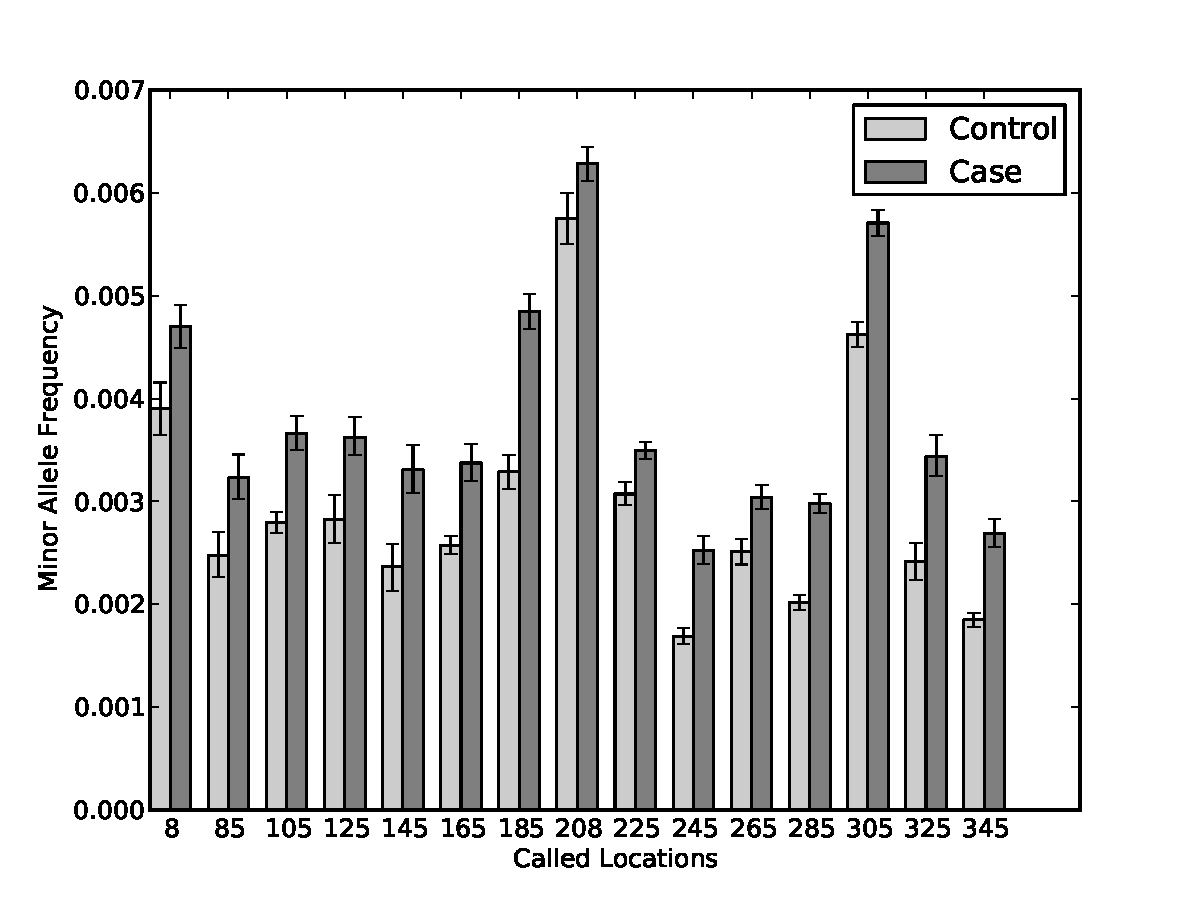
\includegraphics[width=120mm]{pdf_figs/MuBarPlot.pdf}
\caption{Estimated minor allele fraction for called variants in 0.1\% dilution.}
\label{fig:MAF}
\end{center}
\end{figure}


\subsection{Empirical performance compared with other algorithms}\label{sec:comparison}

We compare the empirical performance of RVD2 to other variant calling algorithms. We use the synthetic DNA data sets described in the previous section to explore performance across a dynamic range of read depths as well as minor-allele frequencies. We report the sensitivity and specificity of each algorithm to detect the 14 true positive variant positions out of 400 tested positions.

GATK, samtools and VarScan2-mpileup are optimized to call genotypes on pure samples. Therefore, we expect those algorithms to perform well on the 100\% dilution (pure mutant) sample and poorly on heterogeneous samples. \citet{Stead:2013fu} showed that varscan-somatic outperformed Strelka had performance on-par with muTect in detecting a 5\% MAF for read depths between 100 and 1000. We find its performance on much lower MAF variants and across a wider range of coverage depths. Varscan2-somatic, streak and muTect do not accept replicate data for the ``normal" or ``tumor" bam files so we used a single bam file from each replicate group with a read depth that most closely matched the median overall median depth of the replicates.

Table~\ref{t/l:comparison} shows the sensitivity and specificity for other variant calling algorithms. We computed the Matthews Correlation Coefficient (MCC) as a combined performance measure and present those results in Appendix B~\cite{}. Each cell contains the sensitivity and specificity of the method separated by a slash. The standard genotype variant calling algorithms: samtools, GATK, and VarScan2-mpileup are shown in the first columns. Samtools performs very well on 100\% MAF sample and has nearly perfect sensitivity and specificity for median coverage depths of 27 and 298. 

\begin{figure}[h]
\begin{center}
\includegraphics[width=140mm]{pdf_figs/comparison_table.pdf}
\caption{Comparison of RVD2 with other variant calling algorithms (sensitivity / specificity).}
\label{fig:comparison}
\end{center}
\end{figure}

VarScan2-somatic has perfect performance on a 100\% MAF samples at a low depth. As the depth increases, it calls more false positives and the specificity decreases monotonically from 1.0 to 0.31. For MAFs between 0.1\% and 10\% specificity generally decreases with read depth similarly. There appears to be an optimal read depth for sensitivity. The 100\% MAF sample shows optimal sensitivity at a depth of 27, the 10\% optimal depth is 260 and the 1\% optimal depth is 5584. One would expect that increasing the read depth would lead to better sensitivity, but contrary to expectation further increasing the depth decreases performance. This effect is not exclusive to VarScan2-somatic and is also observed in samtools and GATK. 

Strelka has better sensitivity and specificity than the samtools, GATK or Varscan2-somatic algorithms for almost all read depths and the 100\% and 10\% MAF. However, it has zero sensitivity to detect variants at or below 1\% MAF. 

MuTect has the best overall performance of the other algorithms we tested over a wide range of MAF and depths. Unlike several of the other algorithms muTect generally improves with a higher read depth or the specificity degradation due to false positives is modest. Specifically, muTect calls some of the true variant positions with a 0.3\% MAF and a median read depth of only 53 and 410.

We tested our model RVD2 using two variations of the hypothesis test. We set $\tau$, the hypothesis test threshold to the naive value of zero and we optimized $\tau$ for the read depth and MAF ($\tau^*$). These optimal values were computed from this data set, but in general may be computed once and used as a lookup table for future experiments. With $\tau=0$, RVD2 is not able to call variants with a MAF of 0.1\% if the read depth is less than 4,129. This generally agrees with previous observations and intuition that more than 1,000 reads are required to call a 1:1000 MAF. The specificity degrades slightly at higher read depths with this fixed $\tau$ in line with muTect. At high read depths and MAFs classification is perfect. With $\tau$ set to the optimal value $\tau^*$, we find a significant improvement in both sensitivity and specificity. The algorithm is able to call a 0.1\% MAF with a median read depth of only 39. This performance is due to two properties: (1) the empirical Bayes structure of the model allows parameters $\mu_j$ to borrow strength from one another through $\mu_0$ and (2) the actual coverage at a particular location may be higher than the median coverage across all locations.

\subsection{Pooled Multiple-Sclerosis Samples}\label{sec:ms}

We tested our algorithm on data from pooled samples from patients with multiple-sclerosis (MS). The MS patients are ``high-burden"; meaning that they are known to carry one or more of several genetic risk alleles. Our aim in studying this  patient population is to identify rare risk alleles that may not yet be known to be associated with MS. 

DNA was extracted from whole blood samples from 100 patients with multiple sclerosis and 100 unaffected, unrelated individuals. Each sample was subjected to targeted PCR amplification of IL2RA and interleukin 7 receptor (IL7R); genes with known risk alleles~\cite{HauserNEJM2007}. We targeted X exons covering XXbp in IL2RA and X exon covering XXbp in IL7R. The experiment was repeated on two independent cohorts to filter for spurious associations due to population sampling.

We took 4000 samples from the Markov chain, removed the first 10\% for burn-in and thinned the chain by a factor of 2. We used 10 Metropolis samples for each Gibbs step. We called variants with $\tau = 0.005$ and $\alpha = 0.05$ because we expect that the minimum detectable genotype is a heterozygous mutation in 1 out of 100 samples. 

We identified by consensus of the two independent cohorts two variants in IL7R and one variant in IL2RA. All position information is referenced to human genome reference hg19. One variant in IL7R is rs1494558 at chr5:35861068 T$>$C and has a MAF of 76\% and 71\% in the two cohorts. This mutation causes a missense variant Ile66Thr and has been shown to be associated with abnormal T-cell response and IgA neuropathy~\citep{Hahn:2009bi}. The second IL7R variant is at chr5:35875593 A$>$T and has a MAF of 60\% and 55\% in the two cohorts. This variant has not yet been shown to be associated with any known disease. The IL2RA variant is at chr10:6061965 A$>$T and has a MAF  of 3\% and 5\% in the two cohorts. This variant has not yet been shown to be associated with any known disease.

\begin{figure}[h]
\begin{center}
%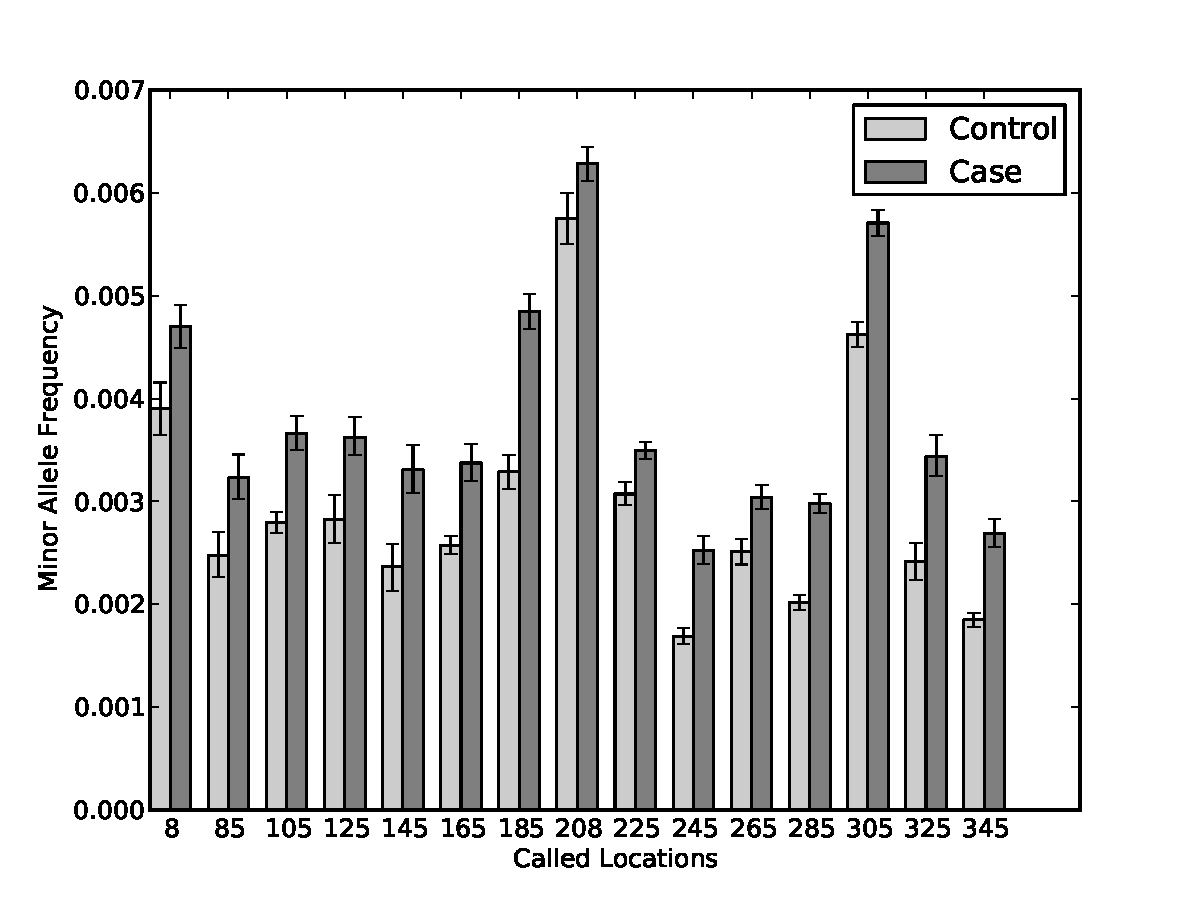
\includegraphics[width=80mm]{pdf_figs/MuBarPlot.pdf}
\caption{Estimated minor allele fractions for consensus variants in MS patient pools.}
\label{fig:MS_MAF}
\end{center}
\end{figure}

The validity of these loci are subject to confirmation on a larger independent sample. However, we note that most GWAS studies focus on common SNPs due to the cost-effective microarray technology used for those studies. We have instead used sequencing technology which yields and unbiased coverage of the targeted regions and has the potential to uncover rare variants that are not targeted by microarray technology. Indeed, the common SNP that was found is associated with an autoimmune disorder and the other two variants are not at dbSNP loci.

\appendix
\section{Parameter Initialization}\label{sec:appendix_mom}
Since $r_{ji} \thicksim \text{Binomial}(n_{ji}, \theta_{ji})$, the first population moment is  $E[r_{ji}] = \theta_{ji} n_{ji}$ and the first sample moment is simply $m_1 = r_{ji}$. Therefore the MoM estimator is 
\begin{equation}
	\tilde{\theta}_{ji} = \frac{r_{ji}} {n_{ji}}
\end{equation}

We take the MoM estimate, $\tilde{\theta}_{ji}$, as data for the next conditional distribution in the hierarchical model. The distribution is $\theta_{ji} \thicksim \text{Beta}(\mu_jM_j, (1-\mu_j)M_j)$. The first and second population moments are
\begin{eqnarray}
	E[\theta_{ji}] =& \mu_j,\\
	\text{Var}[\theta_{ji}] =& \frac{\mu_j(1-\mu_j)} { M_j + 1 }.
\end{eqnarray}
The first and second sample moments are $m_1 = \frac{1}{N}\sum_{i=1}^N \theta_{ji}$ and $m_2 = \frac{1}{N}\sum_{i=1}^N \theta_{ji}^2$. Setting the population moments equal to the sample moments and solving for $\mu_j$ and $M_j$ gives
\begin{eqnarray}
	\tilde{\mu}_j =& \frac{1}{N} \sum_{i=1}^N \theta_{ji}, \\
	\tilde{M_j} =& \frac{ \tilde{\mu}_j (1 - \tilde{\mu}_j ) } { \frac{1}{N} \sum_{i=1}^N \theta_{ji}^2 } -1.
\end{eqnarray}

Following the same procedure for the parameters of $\mu_j \thicksim \text{Beta}(\mu_0, M_0)$ gives the following MoM estimates
\begin{eqnarray}
	\tilde{\mu}_0 =& \frac{1}{J} \sum_{j=1}^J \mu_j \\
	\tilde{M}_0 =& \frac{ \tilde{\mu}_0 (1 - \tilde{\mu}_0 ) } {\frac{1}{J} \sum_{j=1}^J \mu_j^2 } -1.
\end{eqnarray}

\section{Comparison to other algorithms}\label{sec:app_comparison}
\begin{figure}[h]
\begin{center}
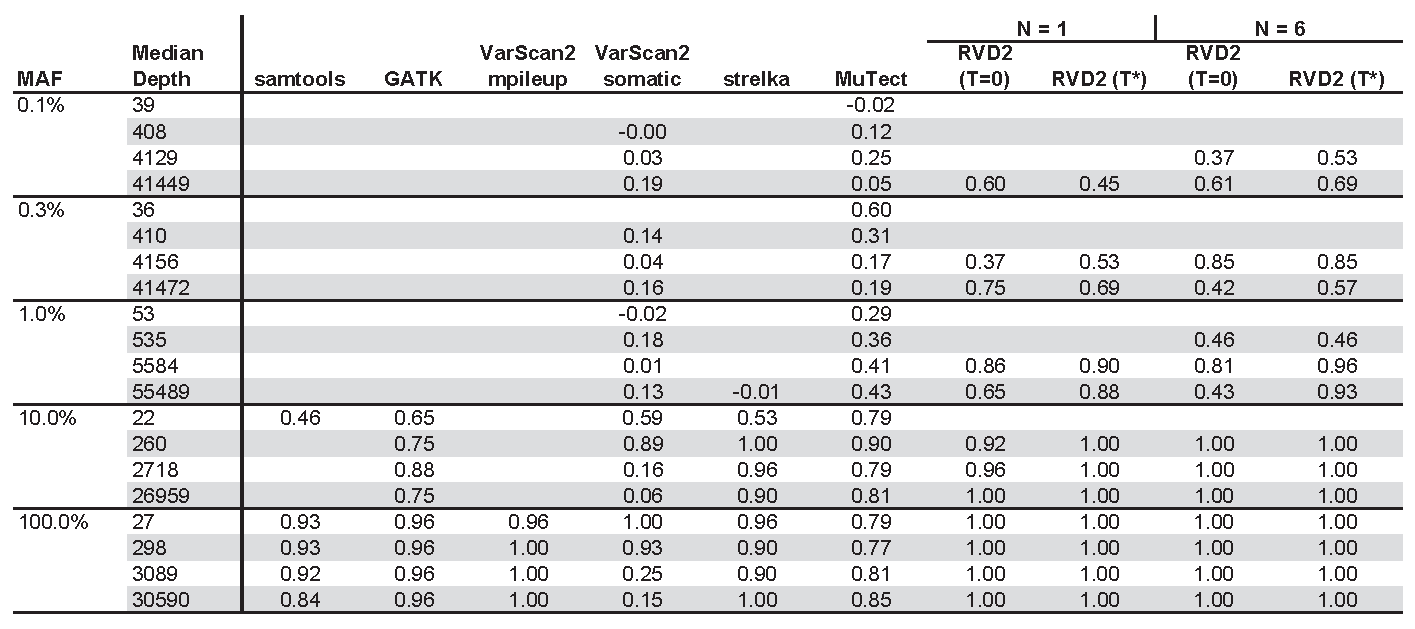
\includegraphics[width=140mm]{pdf_figs/comparison_table_mcc.pdf}
\caption{Comparison of RVD2 with other variant calling algorithms (MCC).}
\label{fig:comparison_mcc}
\end{center}
\end{figure}


\bibliographystyle{apalike}
\bibliography{bioinfo}
\end{document}  
